\documentclass[aspectratio=169, table, 12pt]{beamer}

\usepackage{colortbl}
\usepackage{xcolor}
\usepackage{listings}
\usepackage{tabularx}
\usepackage{tikz}
\usetikzlibrary{arrows.meta, positioning, calc, fit, shapes.geometric}

\makeatletter
\def\input@path{{../theme/}}
\makeatother
\graphicspath{{../theme/}{../../figures/}}
\usetheme{Pradita}

\definecolor{praditagreen}{RGB}{37, 113, 71}

% Tema membuat garis tabel berwarna putih. Dikembalikan agar tabel terbaca.
\arrayrulecolor{black}
\setlength{\arrayrulewidth}{0.5pt}

% Menempatkan gambar di tengah kolom, mendatar sekaligus tegak. Lebarnya
% dipenuhi selebar kolom. Bila hasilnya melebihi tinggi yang disediakan,
% tingginya yang menjadi pembatas, sehingga gambar tidak menembus bingkai.
\newsavebox{\kotakkolom}
\newcommand{\gambarkolom}[2][0.72\textheight]{%
  \sbox{\kotakkolom}{\resizebox{\linewidth}{!}{#2}}%
  \begin{minipage}[c][#1][c]{\linewidth}%
    \centering
    \ifdim\dimexpr\ht\kotakkolom+\dp\kotakkolom\relax>#1\relax
      \resizebox{!}{#1}{#2}%
    \else
      \usebox{\kotakkolom}%
    \fi
  \end{minipage}%
}

\lstdefinestyle{PythonStyle}{
  language=Python,
  basicstyle=\ttfamily\scriptsize,
  keywordstyle=\color{blue}\bfseries,
  commentstyle=\color{gray}\itshape,
  stringstyle=\color{red},
  breaklines=true,
  frame=lines,
  backgroundcolor=\color{lightgray!10},
  tabsize=2,
  showstringspaces=false
}

\lstdefinelanguage{bash}{
  keywords={},
  basicstyle=\ttfamily\scriptsize,
  ndkeywords={cd, python, bash, source, curl},
  ndkeywordstyle=\color{purple}\bfseries,
  sensitive=true,
  commentstyle=\color{gray},
  breaklines=true,
  frame=lines,
  backgroundcolor=\color{lightgray!10},
  tabsize=2,
  comment=[l]{\#},
  showstringspaces=false
}

\title{\Huge{Service-Based Architecture}}
\subtitle{IF231303 Arsitektur Perangkat Lunak}
\author{Alfa Yohannis}

\begin{document}

\frame{\titlepage}

\begin{frame}{{\Large Tujuan Pembelajaran}}
  \vspace{10pt}
  \begin{enumerate}
    \item Menjelaskan tiga ciri service-based architecture, yaitu layanan
          berbutir kasar, basis data bersama, dan gerbang antarmuka.
    \item Membedakan pembagian berbutir kasar tersebut dari monolit berlapis
          maupun dari mikroservis, lalu menentukan kapan masing-masing layak
          dipilih.
    \item Mengukur tambahan waktu tanggap akibat lompatan jaringan, permintaan
          yang selamat ketika satu layanan mati, dan biaya mengubah skema
          basis data bersama.
  \end{enumerate}

  \vspace{10pt}
  {\small Bab ini menempati ruang antara monolit dan mikroservis, yaitu bentuk
  yang paling sering ditemui pada sistem nyata.}
\end{frame}

\begin{frame}{{\Large Pendahuluan}}
  \vspace{8pt}
  \begin{itemize}\small
    \item Pemecahan aplikasi sering dibicarakan sebagai pilihan antara dua
          ujung saja, yaitu monolit dan mikroservis.
    \item Service-based architecture menempati ruang antara keduanya, dengan
          empat sampai duabelas layanan domain.
    \item Setiap layanan berjalan sebagai proses tersendiri dan dipanggil
          lewat HTTP.
    \item Basis datanya tetap satu dan dipakai bersama, dan ciri itulah yang
          membedakannya dari mikroservis.
  \end{itemize}

  \vspace{8pt}
  {\small Harganya dapat diukur dari tiga arah, yaitu waktu tanggap, ketahanan
  terhadap kegagalan, dan biaya perubahan.}
\end{frame}

\begin{frame}{{\Large Butir Layanan yang Kasar}}
  \vspace{6pt}
  \centering
  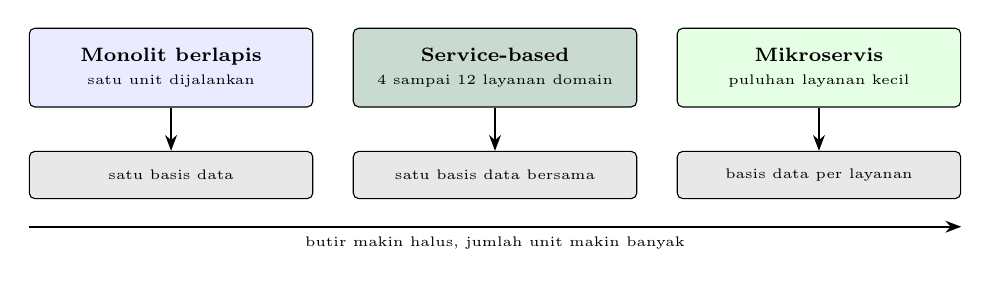
\begin{tikzpicture}[
    kotak/.style={draw, rounded corners=2pt, minimum width=3.6cm,
      minimum height=1.0cm, align=center, font=\scriptsize\bfseries},
    data/.style={draw, rounded corners=2pt, minimum width=3.6cm,
      minimum height=0.6cm, align=center, font=\tiny},
    panah/.style={-{Stealth[length=2mm]}, thick}
  ]
    \node[kotak, fill=blue!8] (mono) {Monolit berlapis\\
      {\tiny\mdseries satu unit dijalankan}};
    \node[kotak, fill=praditagreen!25, right=0.5cm of mono] (layanan)
      {Service-based\\
      {\tiny\mdseries 4 sampai 12 layanan domain}};
    \node[kotak, fill=green!10, right=0.5cm of layanan] (mikro)
      {Mikroservis\\
      {\tiny\mdseries puluhan layanan kecil}};
    \node[data, fill=gray!18, below=0.55cm of mono] (dmono) {satu basis data};
    \node[data, fill=gray!18, below=0.55cm of layanan] (dlayanan)
      {satu basis data bersama};
    \node[data, fill=gray!18, below=0.55cm of mikro] (dmikro)
      {basis data per layanan};
    \draw[panah] (mono) -- (dmono);
    \draw[panah] (layanan) -- (dlayanan);
    \draw[panah] (mikro) -- (dmikro);
    \draw[panah] ([yshift=-0.35cm]dmono.south west)
      -- node[below, font=\tiny] {butir makin halus, jumlah unit makin banyak}
      ([yshift=-0.35cm]dmikro.south east);
  \end{tikzpicture}

  \vspace{6pt}
  {\small Service-based architecture memecah prosesnya, tetapi belum memecah
  basis datanya.}
\end{frame}

\begin{frame}{{\Large Beda dari Kedua Tetangganya}}
  \vspace{8pt}
  \centering
  \small
  \begin{tabularx}{0.95\textwidth}{|l|X|X|X|}
    \hline
    \textbf{Yang dibandingkan} & \textbf{Monolit berlapis} & \textbf{Service-based} & \textbf{Mikroservis} \\
    \hline
    Unit yang dijalankan & Satu & Empat sampai duabelas & Puluhan \\
    \hline
    Basis data & Satu & Satu, dipakai bersama & Terpisah per layanan \\
    \hline
    Pemanggilan antar bidang & Pemanggilan fungsi & Lewat jaringan & Lewat jaringan \\
    \hline
    Yang menjadi mahal & Menjalankan ulang seluruhnya & Mengubah skema bersama & Menjaga data tetap padu \\
    \hline
  \end{tabularx}

  \vspace{8pt}
  {\small Baris terakhir yang paling menentukan. Mikroservis memutus hubungan
  lewat basis data, lalu membayarnya dengan pekerjaan lain.}
\end{frame}

\begin{frame}[fragile]{{\Large Monolit: Pemanggilan Fungsi}}
  \vspace{4pt}
  {\small Ketiga bidang berada di dalam satu proses di porta 8000. Jalur
  gabungannya tiga baris saja.}
  \vspace{2pt}
\begin{lstlisting}[style=PythonStyle]
@aplikasi.post("/pesanan/<int:nomor>/tagihan")
def terbitkan_tagihan(nomor: int) -> dict:
  pesanan = domain_pemesanan.ambil_pesanan(nomor)
  kurs = domain_kurs.ambil_kurs(pesanan["mata_uang"])
  tagihan = domain_penagihan.terbitkan_tagihan(nomor, kurs["nilai"])
  return {"pesanan": pesanan, "kurs": kurs, "tagihan": tagihan,
          "lompatan": alamat.LOMPATAN_KLIEN}
\end{lstlisting}
  \vspace{2pt}
  {\small Tidak ada permintaan yang perlu disusun, tidak ada jawaban yang
  perlu diuraikan, dan lompatan jaringannya satu.}
\end{frame}

\begin{frame}{{\Large Gerbang, Layanan, Basis Data}}
  \vspace{2pt}
  \begin{columns}[c]
    \begin{column}{0.54\textwidth}
      \gambarkolom{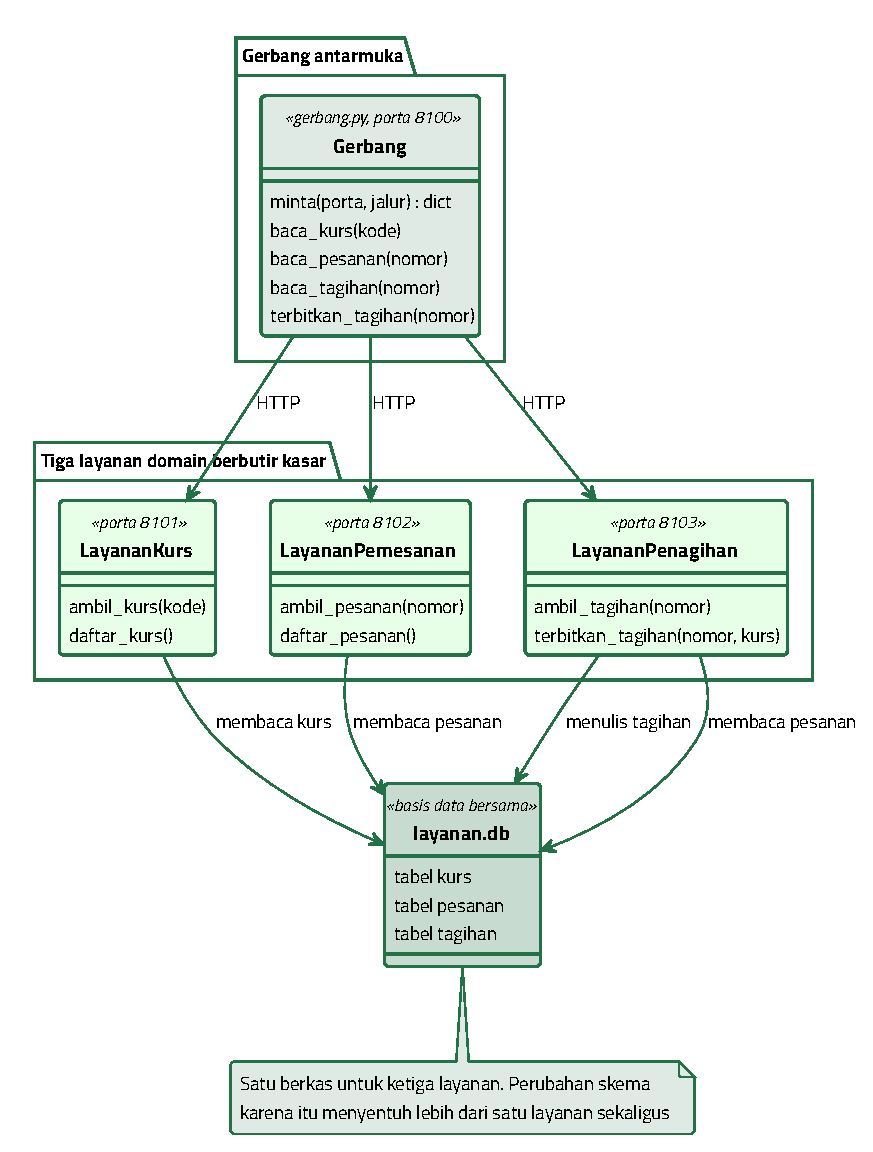
\includegraphics{kelas-layanan.pdf}}
    \end{column}
    \begin{column}{0.44\textwidth}
      \begin{itemize}\small
        \item Gerbang di porta 8100, tanpa satu pun aturan bisnis.
        \item Ketiga layanan domain di porta 8101, 8102, dan 8103.
        \item Ketiganya menunjuk berkas basis data yang sama.
        \item Layanan penagihan menulis tabel tagihan sekaligus membaca tabel
              pesanan.
      \end{itemize}
    \end{column}
  \end{columns}
\end{frame}

\begin{frame}[fragile]{{\Large Service-Based: Tiga Panggilan}}
  \vspace{4pt}
\begin{lstlisting}[style=PythonStyle]
@aplikasi.post("/pesanan/<int:nomor>/tagihan")
def terbitkan_tagihan(nomor: int) -> dict:
  pesanan = minta(alamat.PORTA_PEMESANAN, f"/pesanan/{nomor}")
  kurs = minta(alamat.PORTA_KURS, f"/kurs/{pesanan['mata_uang']}")
  tagihan = minta(alamat.PORTA_PENAGIHAN, f"/tagihan/{nomor}", "POST",
                  {"nilai_kurs": kurs["nilai"]})
  return {"pesanan": pesanan, "kurs": kurs, "tagihan": tagihan,
          "lompatan": (alamat.LOMPATAN_KLIEN + pesanan["lompatan"]
                       + kurs["lompatan"] + tagihan["lompatan"])}
\end{lstlisting}
  \vspace{2pt}
  {\small Ketiganya berurutan, sebab nilai kurs baru diketahui sesudah
  pesanannya terbaca. Angka lompatan dijumlahkan dari jawaban setiap layanan,
  bukan ditulis sebagai tetapan.}
\end{frame}

\begin{frame}{{\Large Urutan pada Kedua Versi}}
  \vspace{4pt}
  \begin{center}
    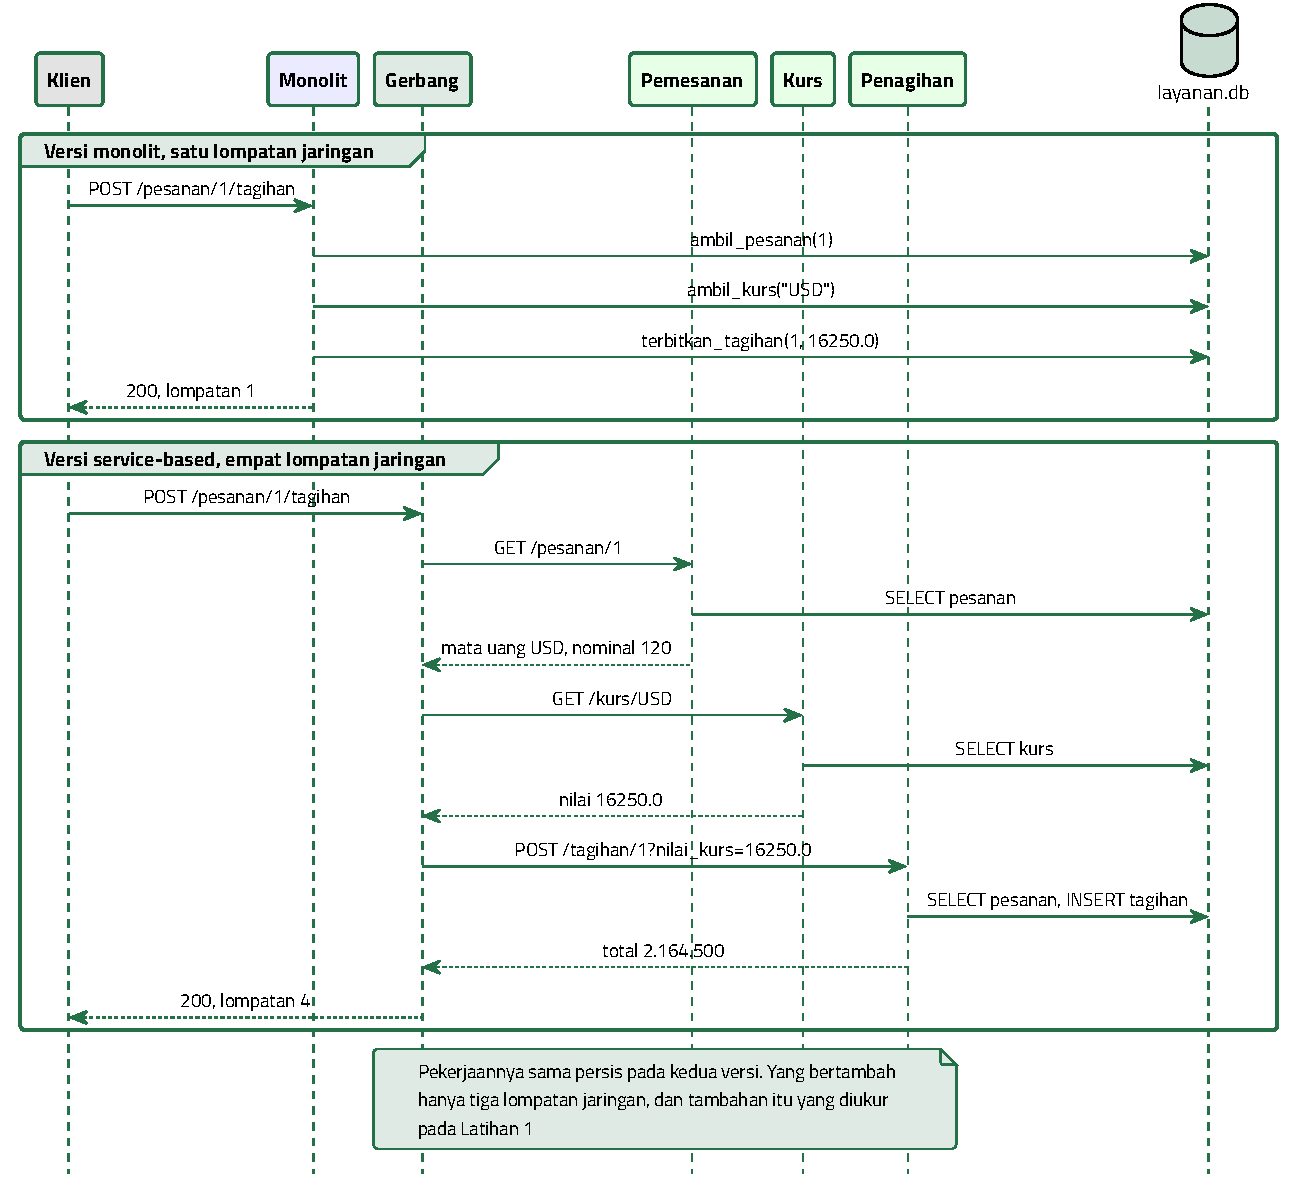
\includegraphics[width=\textwidth, height=0.56\textheight,
      keepaspectratio]{sekuens-layanan.pdf}
  \end{center}
  {\small Pekerjaannya sama persis. Yang bertambah hanya tiga lompatan
  jaringan, yaitu satu melawan empat.}
\end{frame}

\begin{frame}[fragile]{{\Large Pembacaan Silang Antar Bidang}}
  \vspace{4pt}
\begin{lstlisting}[style=PythonStyle]
AMBIL_PESANAN_UNTUK_TAGIHAN = """
SELECT nomor, nominal, status
FROM pesanan
WHERE nomor = ?
"""
    if baris["status"] == basis_data.STATUS_BATAL:
      raise kesalahan.AturanDilanggar(
        f"pesanan {nomor_pesanan} sudah dibatalkan, tidak dapat ditagih")
\end{lstlisting}
  \vspace{2pt}
  \begin{itemize}\small
    \item Bidang penagihan membaca tabel pesanan langsung, bukan bertanya
          kepada bidang pemesanan.
    \item Murah dan menggoda, sebab satu kueri sudah cukup.
    \item Akibatnya, nama kolom pada tabel pesanan kini dipakai dua bidang
          sekaligus.
  \end{itemize}
\end{frame}

\begin{frame}{{\Large Analogi: Tiga Loket, Satu Lemari}}
  \vspace{10pt}
  \begin{itemize}\small
    \item Kantor layanan mahasiswa punya tiga loket, yaitu keuangan,
          akademik, dan kemahasiswaan.
    \item Ketiga loket melayani antrean sendiri-sendiri, sehingga loket yang
          tutup tidak menghentikan loket sebelahnya.
    \item Berkas mahasiswa tetap disimpan di satu lemari arsip di belakang
          ruangan.
    \item Ketiga petugas mengambil dari lemari yang sama.
  \end{itemize}

  \vspace{10pt}
  {\small Menutup satu loket memotong satu antrean. Mengunci lemari arsip
  menghentikan ketiga loket sekaligus.}
\end{frame}

\begin{frame}{{\Large Kasus: Satu Kolom Diganti Namanya}}
  \vspace{8pt}
  \begin{enumerate}\small
    \item Sebuah tim memecah sistem pembayaran kampus menjadi empat layanan
          dengan satu basis data.
    \item Pada suatu malam, kolom \texttt{nominal} pada tabel pesanan diganti
          menjadi \texttt{nominal\_asing}.
    \item Perubahan itu dijalankan bersama pembaruan layanan pemesanan saja.
    \item Layanan penagihan masih memuat kueri lama yang menyebut kolom lama.
  \end{enumerate}

  \vspace{8pt}
  {\small Kegagalan baru ketahuan keesokan paginya, yaitu ketika tagihan
  pertama diterbitkan. Pembaruan satu layanan terpaksa ditarik kembali,
  padahal kodenya sendiri tidak bersalah.}
\end{frame}

\begin{frame}{{\Large Hasil Pengukuran: Waktu Tanggap}}
  \vspace{8pt}
  \centering
  \small
  \begin{tabularx}{0.9\textwidth}{|X|l|l|}
    \hline
    \textbf{Yang diukur} & \textbf{Monolit} & \textbf{Service-based} \\
    \hline
    Median & 5,03 ms & 9,07 ms \\
    \hline
    Persentil ke-95 & 5,87 ms & 10,89 ms \\
    \hline
    Terbesar & 9,74 ms & 29,68 ms \\
    \hline
    Lompatan jaringan per permintaan & 1 & 4 \\
    \hline
    Putaran lebih cepat & 150 dari 150 & 0 dari 150 \\
    \hline
  \end{tabularx}

  \vspace{8pt}
  {\small \textit{Range} jalur monolit 5,20 ms, yaitu 1,29 kali selisih
  mediannya. Yang menggelembungkannya satu putaran lambat, sedangkan
  persentil ke-95 kedua jalur tidak bertumpang tindih.}
\end{frame}

\begin{frame}{{\Large Hasil: Satu Bagian Dimatikan}}
  \vspace{8pt}
  \centering
  \small
  \begin{tabularx}{0.9\textwidth}{|X|l|l|}
    \hline
    \textbf{Keadaan} & \textbf{Monolit} & \textbf{Service-based} \\
    \hline
    Seluruh proses hidup & 4 dari 4 & 4 dari 4 \\
    \hline
    Bidang kurs dimatikan & 0 dari 4 & 2 dari 4 \\
    \hline
    Basis data bersama dikunci & 0 dari 4 & 0 dari 4 \\
    \hline
  \end{tabularx}

  \vspace{8pt}
  {\small Yang selamat pada baris kedua adalah baca pesanan dan baca tagihan.
  Baris ketiga memperlihatkan batasnya, sebab memecah proses tidak dengan
  sendirinya memecah titik kegagalan.}
\end{frame}

\begin{frame}{{\Large Hasil Pengukuran: Biaya Perubahan}}
  \vspace{8pt}
  \centering
  \small
  \begin{tabularx}{0.9\textwidth}{|X|l|l|}
    \hline
    \textbf{Yang dihitung} & \textbf{Monolit} & \textbf{Service-based} \\
    \hline
    Fitur satu bidang, berkas berubah & 2 & 2 \\
    \hline
    Fitur satu bidang, proses ulang & 1 dari 1 & 1 dari 4 \\
    \hline
    Skema bersama, berkas berubah & 3 & 3 \\
    \hline
    Skema bersama, baris berubah & 16 & 16 \\
    \hline
    Skema bersama, proses ulang & 1 dari 1 & 3 dari 4 \\
    \hline
  \end{tabularx}

  \vspace{8pt}
  {\small Kedua baris proses ulang berlawanan arah. Layanan kurs pun ikut
  dijalankan ulang, sebab layanan itu memuat berkas tempat skema disimpan.}
\end{frame}

\begin{frame}{{\Large Ringkasan}}
  \vspace{10pt}
  \begin{itemize}\small
    \item Layanan berbutir kasar, lazimnya empat sampai duabelas, dipanggil
          lewat jaringan, dengan satu basis data bersama.
    \item Aturan lintas bidang tetap dapat ditulis sebagai satu kueri, sebab
          basis datanya memang belum dipisah.
    \item Yang dibayar adalah waktu tanggap, yaitu median 1,8 kali lebih lama
          dengan empat lompatan melawan satu.
    \item Kegagalan tertahan sejauh prosesnya saja, sebab basis data bersama
          menjatuhkan kedua versi sekaligus.
  \end{itemize}

  \vspace{10pt}
  {\small Pesan utamanya bukan bahwa layanan harus dipecah, melainkan bahwa
  setiap pemecahan menentukan perubahan mana yang murah.}
\end{frame}

\begin{frame}[fragile]{{\Large Persiapan Latihan}}
  \vspace{5pt}
\begin{lstlisting}[language=bash]
bash sources/siapkan_venv.sh
source .venv/bin/activate
cd sources/chapter11
python basis_data.py
# Basis data bersama : layanan.db
python jalankan_layanan.py
# Terlayani monolit       : 4 dari 4
# Terlayani service-based : 4 dari 4
\end{lstlisting}

  \vspace{6pt}
  {\small Perintah terakhir menyalakan kelima proses, mencoba empat jenis
  permintaan pada kedua versi, lalu mematikan seluruhnya. Untuk membiarkannya
  hidup, jalankan \texttt{python jalankan\_layanan.py hidup}.}
\end{frame}

\begin{frame}[fragile]{{\Large Latihan 1: Tambahan Lompatan}}
  \vspace{3pt}
\begin{lstlisting}[language=bash]
python ukur_latensi.py
# Median monolit                : 5.03 ms
# Median service-based          : 9.07 ms
# Putaran monolit lebih cepat   : 150 dari 150
\end{lstlisting}

  \vspace{3pt}
  \begin{enumerate}\small
    \item Catat median, persentil ke-95, dan nilai terbesar kedua versi.
    \item Catat kedua angka lompatan beserta pencacahan putarannya.
    \item Hitung berapa kali fungsi \texttt{minta} dipanggil pada jalur
          terbitkan tagihan, lalu bandingkan dengan angka lompatannya.
  \end{enumerate}

  \vspace{3pt}
  {\small Pertanyaan: mengapa selisihnya layak disebut ada walaupun
  \textit{range} jalur monolit lebih besar daripada selisih itu sendiri?}
\end{frame}

\begin{frame}[fragile]{{\Large Latihan 2: Mematikan Satu Layanan}}
  \vspace{3pt}
\begin{lstlisting}[language=bash]
python uji_kegagalan.py
# Bidang kurs dimatikan          0 dari 4    2 dari 4
# Basis data bersama dikunci     0 dari 4    0 dari 4
\end{lstlisting}

  \vspace{3pt}
  \begin{enumerate}\small
    \item Catat ketiga baris ringkasan beserta nama permintaan yang masih
          terlayani.
    \item Tunjukkan baris pada \texttt{uji\_kegagalan.py} yang mematikan satu
          layanan saja.
    \item Ubah \texttt{LAYANAN\_DIMATIKAN} menjadi \texttt{"pemesanan"},
          jalankan ulang, lalu catat perubahan angkanya.
  \end{enumerate}

  \vspace{3pt}
  {\small Pertanyaan: apa yang dibuktikan baris basis data terkunci tentang
  batas pemecahan proses?}
\end{frame}

\begin{frame}[fragile]{{\Large Latihan 3: Mengubah Skema Bersama}}
  \vspace{3pt}
\begin{lstlisting}[language=bash]
python biaya_perubahan.py
# Service-based  berkas 3   baris 16   proses ulang 3 dari 4
# Proses ulang   : kurs, pemesanan, penagihan
\end{lstlisting}

  \vspace{3pt}
  \begin{enumerate}\small
    \item Catat keenam angka pada kedua bagian laporannya.
    \item Baca isi \texttt{PERUBAHAN} untuk melihat penggantian teks yang
          dipakainya.
    \item Terapkan perubahan kedua sungguhan, lalu catat apa yang terjadi bila
          hanya satu dari ketiga berkas yang diubah.
  \end{enumerate}

  \vspace{3pt}
  {\small Pertanyaan: dengan menggabungkan hasil ketiga latihan, kapan
  pembagian berbutir kasar ini lebih tepat daripada monolit maupun
  mikroservis?}
\end{frame}

\end{document}
